\documentclass{standalone}
\usepackage{tikz}
\usepackage{pgfplots}
\begin{document}
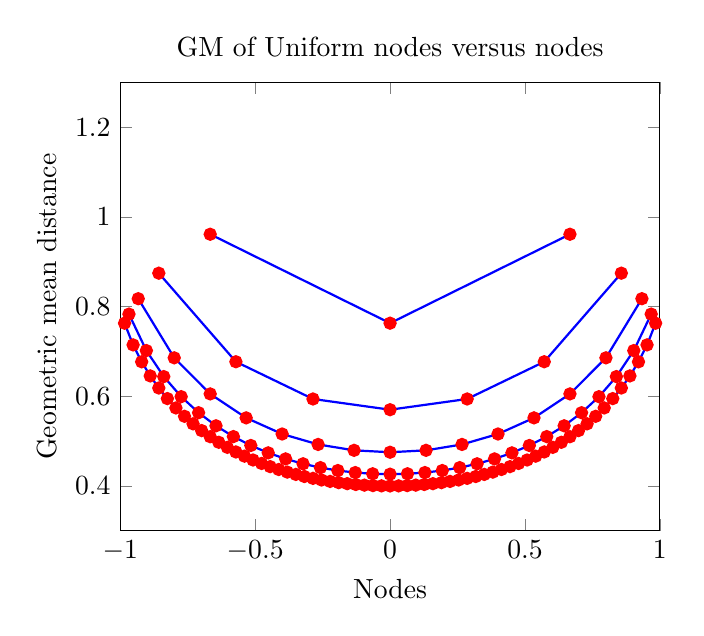
\begin{tikzpicture}
\begin{axis}[
title = GM of Uniform nodes versus nodes,
xlabel = {Nodes},
ylabel = {Geometric mean distance},
xmin	= -1, xmax = 1,
ymin	= 0.3, ymax = 1.3,
legend style ={
at={(0, 0)},
anchor = 
}
]
\addplot[
blue,
,
thick,
mark = *,
mark options = {red, solid,},
] coordinates {
	(-0.666667,0.9615)
	(0,0.763143)
	(0.666667,0.9615)
};
\addplot[
blue,
,
thick,
mark = *,
mark options = {red, solid,},
] coordinates {
	(-0.857143,0.874674)
	(-0.571429,0.677145)
	(-0.285714,0.594064)
	(0,0.570144)
	(0.285714,0.594064)
	(0.571429,0.677145)
	(0.857143,0.874674)
};
\addplot[
blue,
,
thick,
mark = *,
mark options = {red, solid,},
] coordinates {
	(-0.933333,0.81778)
	(-0.8,0.685848)
	(-0.666667,0.605388)
	(-0.533333,0.551946)
	(-0.4,0.51595)
	(-0.266667,0.492651)
	(-0.133333,0.479512)
	(0,0.475263)
	(0.133333,0.479512)
	(0.266667,0.492651)
	(0.4,0.51595)
	(0.533333,0.551946)
	(0.666667,0.605388)
	(0.8,0.685848)
	(0.933333,0.81778)
};
\addplot[
blue,
,
thick,
mark = *,
mark options = {red, solid,},
] coordinates {
	(-0.967742,0.783413)
	(-0.903226,0.702007)
	(-0.83871,0.643988)
	(-0.774194,0.59922)
	(-0.709677,0.563423)
	(-0.645161,0.534242)
	(-0.580645,0.510205)
	(-0.516129,0.490324)
	(-0.451613,0.473902)
	(-0.387097,0.460433)
	(-0.322581,0.449544)
	(-0.258065,0.440958)
	(-0.193548,0.434469)
	(-0.129032,0.429932)
	(-0.0645161,0.427248)
	(0,0.426359)
	(0.0645161,0.427248)
	(0.129032,0.429932)
	(0.193548,0.434469)
	(0.258065,0.440958)
	(0.322581,0.449544)
	(0.387097,0.460433)
	(0.451613,0.473902)
	(0.516129,0.490324)
	(0.580645,0.510205)
	(0.645161,0.534242)
	(0.709677,0.563423)
	(0.774194,0.59922)
	(0.83871,0.643988)
	(0.903226,0.702007)
	(0.967742,0.783413)
};
\addplot[
blue,
,
thick,
mark = *,
mark options = {red, solid,},
] coordinates {
	(-0.984127,0.7631)
	(-0.952381,0.714712)
	(-0.920635,0.676972)
	(-0.888889,0.645534)
	(-0.857143,0.618539)
	(-0.825397,0.594937)
	(-0.793651,0.574052)
	(-0.761905,0.555414)
	(-0.730159,0.538675)
	(-0.698413,0.52357)
	(-0.666667,0.509893)
	(-0.634921,0.497474)
	(-0.603175,0.486179)
	(-0.571429,0.475894)
	(-0.539683,0.466524)
	(-0.507937,0.45799)
	(-0.47619,0.450223)
	(-0.444444,0.443165)
	(-0.412698,0.436766)
	(-0.380952,0.430983)
	(-0.349206,0.425778)
	(-0.31746,0.421119)
	(-0.285714,0.416978)
	(-0.253968,0.413332)
	(-0.222222,0.410159)
	(-0.190476,0.407442)
	(-0.15873,0.405166)
	(-0.126984,0.40332)
	(-0.0952381,0.401894)
	(-0.0634921,0.400881)
	(-0.031746,0.400275)
	(0,0.400073)
	(0.031746,0.400275)
	(0.0634921,0.400881)
	(0.0952381,0.401894)
	(0.126984,0.40332)
	(0.15873,0.405166)
	(0.190476,0.407442)
	(0.222222,0.410159)
	(0.253968,0.413332)
	(0.285714,0.416978)
	(0.31746,0.421119)
	(0.349206,0.425778)
	(0.380952,0.430983)
	(0.412698,0.436766)
	(0.444444,0.443165)
	(0.47619,0.450223)
	(0.507937,0.45799)
	(0.539683,0.466524)
	(0.571429,0.475894)
	(0.603175,0.486179)
	(0.634921,0.497474)
	(0.666667,0.509893)
	(0.698413,0.52357)
	(0.730159,0.538675)
	(0.761905,0.555414)
	(0.793651,0.574052)
	(0.825397,0.594937)
	(0.857143,0.618539)
	(0.888889,0.645534)
	(0.920635,0.676972)
	(0.952381,0.714712)
	(0.984127,0.7631)
};
\legend{};
\end{axis}
\end{tikzpicture}
\end{document}
